\documentclass{article}
\usepackage{graphicx}

%Enumering lower case roman numerals
%\renewcommand{\theenumi}{\roman{enumi}}   
%\renewcommand{\labelenumi}{\theenumi)}


\begin{document}

\title{EE3025 Assignment-2}

\author{C Shruti \\ EE18BTECH11006}

\maketitle
%-------------------------------------------------------------------------------
Download all python codes and latex-tikz codes from 
\begin{verbatim}
https://github.com/shruti-chepuri/EE3025/tree/main/Assignment-2
\end{verbatim}
%
\section{Introduction}
We are supposed to design the equivalent FIR and IIR filter realizations for filter number 114.  
This is a bandpass filter whose specifications are available below.

\section{Filter Specifications}
The sampling rate for the filter has been specified as $F_s =  48$ kHz.	If the un-normalized  discrete-time (natural) frequency is F, the corresponding normalized digital filter (angular) frequency is given by $\omega = 2\pi
\left(\frac{F}{F_s}\right)$.

\subsection{The Digital Filter}

\begin{enumerate}
\item {\em Tolerances:}  The passband ($\delta_1$) and stopband ($\delta_2$) tolerances are given to
be equal, so we let $\delta_1 = \delta_2 = \delta = 0.15$.

\item {\em Passband:}  The passband of filter number $j$, $j$ going from 109 to 135 is from \{3 + 0.6(j-109)\}kHz
to \{3 + 0.6(j-107)\}kHz.  Since our filter number is 114, substituting $j = 114$ gives the passband
range for our bandpass filter as $6$ kHz - $7.2$ kHz.  Hence, the un-normalized discrete time filter
passband frequencies are $F_{p1} = 7.2$ kHz
and $F_{p2} = 6.0$ kHz.  The corresponding normalized digital filter passband frequencies are
$\omega_{p1} = 2\pi\frac{F_{p1}}{F_s}  = 0.3\pi$  and $\omega_{p2} = 2\pi\frac{F_{p2}}{F_s}  = 0.25 \pi$ kHz.  The centre frequency is then given by  $\omega_c = \frac{\omega_{p1} + \omega_{p2}}{2} = 0.275\pi$.  

\item {\em Stopband:}  The {\em transition band} for bandpass filters is $\Delta F = 0.3$ kHz on either side of the passband.
Hence, the un-normalized {\em stopband} frequencies are $F_{s1} = 7.2 + 0.3 = 7.5$ kHz and $F	_{s2} = 6.0 - 0.3 = 5.7$ kHz.  The corresponding normalized frequencies are $\omega_{s1} = 0.3125 \pi$  and $\omega_{s2} =  0.2375 \pi$.
\end{enumerate}

\subsection{The Analog filter}
In the bilinear transform, the analog filter frequency ($\Omega$) is related to the corresponding digital filter frequency ($\omega$) as $\Omega = \tan \frac{\omega}{2}$.  Using this relation, we obtain the analog passband and stopband frequencies as $\Omega_{p1} = 0.5095$, $\Omega_{p2} = 0.4142$ and $\Omega_{s1} = 0.5345$, $\Omega_{s2} = 0.3914$
respectively.

\section{The IIR Filter Design}
{\em Filter Type:}  We are supposed to design filters whose stopband is monotonic and passband equiripple.  
Hence, we use the {\em Chebyschev approximation} to design our bandpass IIR filter.

\subsection{The Analog Filter}
\begin{enumerate}

\item {\em Low Pass Filter Specifications:}  If $H_{a, BP}(j\Omega)$ be the desired analog band
pass filter,  with the specifications provided in Section 2.2, and $H_{a,LP}(j\Omega_L)$ 
be the equivalent low pass filter, then
\begin{equation}
\label{transition}
\Omega_L = \frac{\Omega^2 - \Omega_0^2}{B\Omega}
\end{equation}

%\begin{equation}
%H_{a, BP}(j\Omega) =  H_{a,LP}(j\Omega_L) \vert_{ \Omega_L = 
%\frac{\Omega^2 - \Omega_0^2}{B\Omega}},
%\end{equation}
where $\Omega_0 = \sqrt{\Omega_{p1}\Omega_{p2}} = 0.4594$ and $B = \Omega_{p1} - \Omega_{p2} = 0.0953$.  The low pass filter has
the passband edge at $\Omega_{Lp} = 1$ and stopband edges at $\Omega_{Ls_1} = 1.4653$ and $\Omega_{Ls_2} = -1.5511$.  We choose the stopband edge of the analog low pass filter as $\Omega_{Ls} = \mbox{min}(\vert \Omega_{Ls_1}\vert,\vert \Omega_{Ls_2}\vert) = 1.4653$.

\item {\em The Low Pass Chebyschev Filter Paramters:}  The magnitude squared of the Chebyschev low pass filter is given by 
\begin{equation}
\label{lpfirst}
\vert H_{a,LP}(j\Omega_L)\vert^2 = \frac{1}{1 + \epsilon^2c_N^2(\Omega_L/\Omega_{Lp})}
\end{equation}
where $c_N(x) = \cosh(N \cosh^{-1}x)$ and the integer $N$, which is the order of the filter, and $\epsilon$ are design paramters.  Since $\Omega_{Lp} = 1$, (\ref{lpfirst}) may be rewritten as
\begin{equation}
\label{lpsecond}
\vert H_{a,LP}(j\Omega_L)\vert^2 = \frac{1}{1 + \epsilon^2c_N^2(\Omega_L)}
\end{equation}
Also, the design paramters have the following constraints
\begin{eqnarray}
\label{lpdesign}
\frac{\sqrt{D_2}}{c_N(\Omega_{Ls})} \leq \epsilon \leq \sqrt{D_1}, \nonumber \\
N \geq \left\lceil \frac{\cosh^{-1}\sqrt{D_2/D_1}}{\cosh^{-1}\Omega_{Ls}} \right\rceil,
\end{eqnarray}
where $D_1 = \frac{1}{(1 - \delta)^2}-1$ and $D_2 = \frac{1}{\delta^2} - 1$.  After appropriate substitutions,
we obtain $N \geq 4$ and $0.3184 \leq \epsilon \leq 0.6197$.  In Figure 1, we plot $\vert H(j\Omega)\vert$ for a range of values of $\epsilon$, for $N = 4$.  We find that for larger values of $\epsilon$, $|H(j\Omega)|$ decreases in the transition band.  We choose $\epsilon = 0.4$  for our IIR filter design.  

%For this value of $epsilon$, the plot of $\vert H(j\Omega) \vert$ is shown for various $4 \leq N \leq 10$.  For increasing values of $N$, we find that that fall from the passband to the stopband is sharp.  For $N = 6$, we find that $\vert H(j\Omega_{Ls}) \vert$ is very close to $\delta$, thus meeting the constraints imposed on the magnitude response of the filter.  Based on the above discussion, we choose $N = 6, \epsilon = 0.5$ as the design paramters for the equivalent lowpass Chebyschev approximation.  

\item {\em The Low Pass Chebyschev Filter:} Thus, we obtain
\begin{equation}
\label{lpsqfinal}
\vert H_{a,LP}(j\Omega_L)\vert^2 = \frac{1}{1 + 0.16c_4^2(\Omega_L)}
\end{equation}
where
\begin{equation}
c_4(x) = 8x^4 + 8x^2 + 1.	
\end{equation}
The poles of the frequency response in (\ref{lpfirst}) lying in the left half plane are in general obtained as 
$r_1\cos\phi_k + jr_2\sin \phi_k$, where
\begin{eqnarray}
\label{lppoles}
\phi_k = \frac{\pi}{2} + \frac{(2k+1)\pi}{2N}, k = 0, 1, \dots, N-1 \nonumber \\
r_1 = \frac{\beta^2 - 1}{2\beta}, r_2 = \frac{\beta^2 + 1}{2\beta}, \beta = \left[ \frac{\sqrt{1 + \epsilon^2} + 1}{\epsilon}\right]^{\frac{1}{N}}
\end{eqnarray}
Thus, for N even, the low-pass stable Chebyschev filter, with a gain $G$ has the form
\begin{equation}
\label{poleleft}
H_{a,LP}(s_L) = \frac{G_{LP}}{\prod_{k = 1}^{\frac{N}{2}-1}(s_L^2 - 2r_1\cos\phi_ks_L + r_1^2\cos^2\phi_k + r_2^2 \sin^2\phi_k)}
\end{equation}
Substituting $N = 4$, $\epsilon = 0.5$ and $H_{a,LP}(j) = \frac{1}{\sqrt{1+\epsilon^2}}$, from (\ref{lppoles}) and (\ref{poleleft}), we obtain 
\begin{equation}
\label{lpfinal}
H_{a,LP}(s_L) = \frac{0.3125}{s_L^4 + 1.1068s_L^3 + 1.6125s_L^2+0.9140s_L + 0.3366}
\end{equation}
In Figure 2 we plot $|H(j\Omega)|$ using (\ref{lpsqfinal}) and (\ref{lpfinal}), thereby verifying that our low-pass Chebyschev filter design meets the specifications.
\item {\em The Band Pass Chebyschev Filter:}  The analog bandpass filter is obtained from (\ref{lpfinal}) by substituting
$s_L = \frac{s^2 + \Omega_0^2}{Bs}$.  Hence
\begin{equation}
H_{a,BP}(s) = G_{BP}H_{a,LP}(s_L)\vert_{s_L = \frac{s^2 + \Omega_0^2}{Bs}},
\end{equation}
where $G_{BP}$ is the gain of the bandpass filter.  After appropriate substitutions, and evaluating the gain 
such that $H_{a,BP}(j\Omega_{p1}) = 1$, we obtain
{\tiny
\begin{equation}
\label{bpfinal}
H_{a,BP}(s) = \frac{2.7776\times 10^{-5}s^4}{s^8+0.1055s^7+0.8589s^6+0.0676s^5+0.2735s^4+0.0143s^3+0.0383s^2+0.001s+0.002}
\end{equation}
}
In Figure 3, we plot $\vert H_{a,BP}(j\Omega)\vert$ as a function of $\Omega$ for both positve as
well as negative frequencies.  We find that the passband and stopband frequencies in the figure
match well with those obtained analytically through the bilinear transformation.
\end{enumerate}
\begin{figure}
\label{fig1}
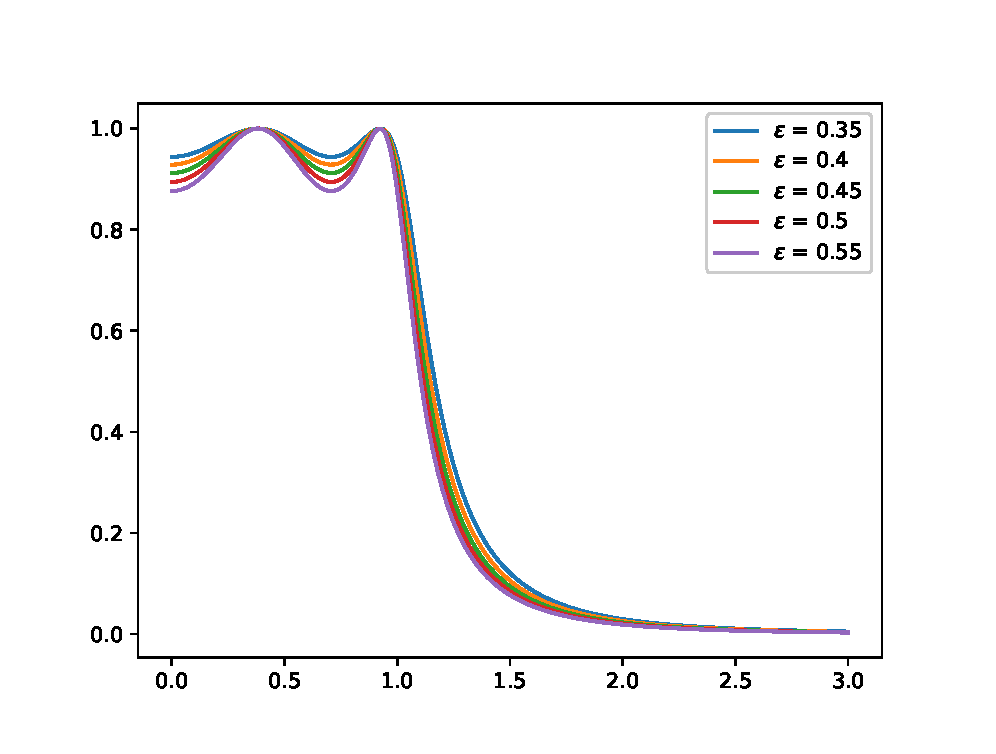
\includegraphics[width = 15cm]{figs/iir/Varying_epsilon.eps}
\caption{The Analog Low-Pass Frequency Response for $0.35 \leq \epsilon \leq 0.6$}
\end{figure}


\begin{figure}
\label{fig2}
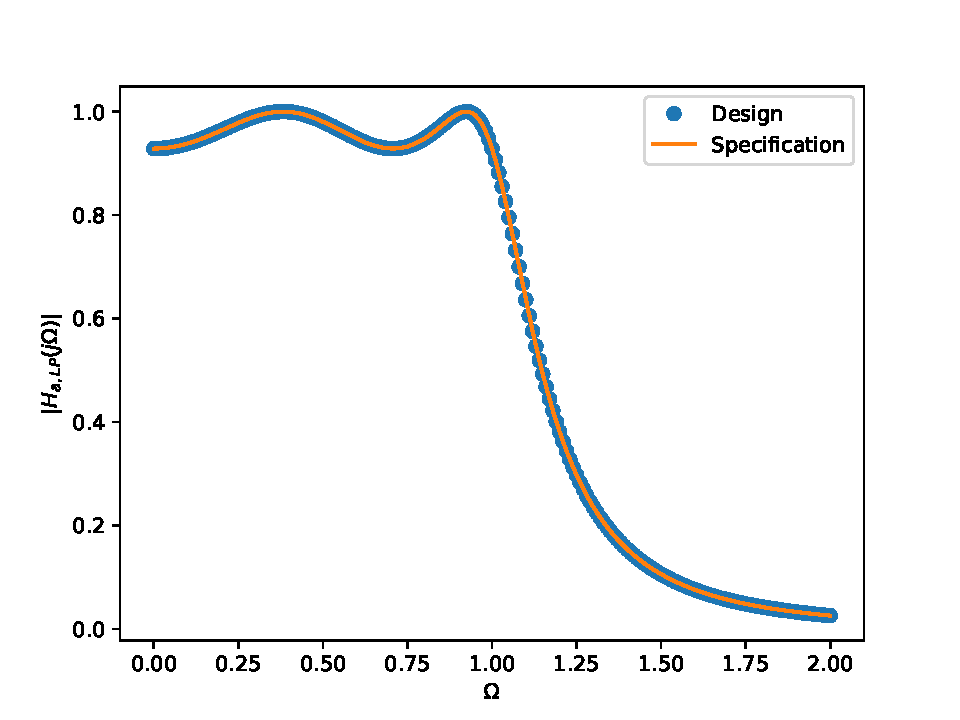
\includegraphics[width = 15cm]{figs/iir/AnalogLP_cheb.eps}
\caption{The magnitude response plots from the specifications in Equation \ref{lpsqfinal} and the design in Equation \ref{lpfinal}}
\end{figure}

\begin{figure}
\label{fig3}
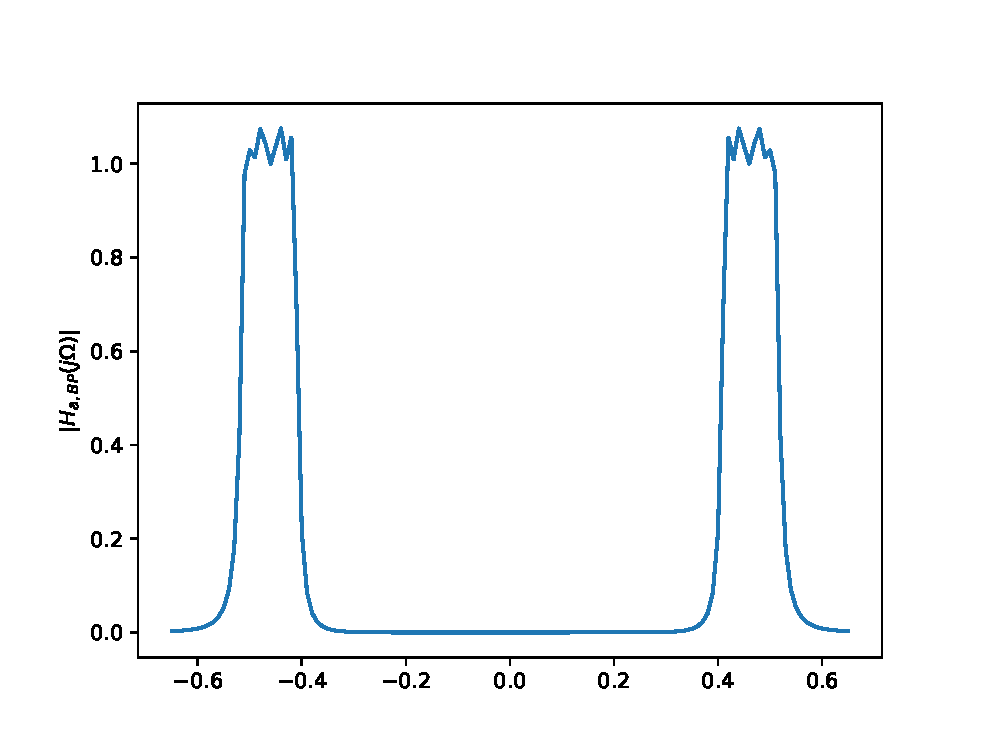
\includegraphics[width = 15cm]{figs/iir/BP_analog.eps}
\caption{The analog bandpass magnitude response plot from Equation \ref{bpfinal}} 
\end{figure}

\subsection{The Digital Filter}
From the bilinear transformation, we obtain the digital bandpass filter from the corresponding analog filter as
\begin{eqnarray}
\label{analdig}
H_{d,BP}(z) = GH_{a,BP}(s)\vert_{s = \frac{1-z^{-1}}{1 + z^{-1}}}
\end{eqnarray}
where $G$ is the gain of the digital filter.  From (\ref{bpfinal}) and (\ref{analdig}), we obtain

\begin{eqnarray}
H_{d,BP}(z) = G \frac{N(z)}{D(z)}
\end{eqnarray}
where $G = 2.7776 \times 10^{-5}$,

\begin{eqnarray}
N(z)=  1 - 4 z^{-2} + 6 z^{-4} - 4z^{-6} + z^{-8} 
\end{eqnarray}
and
\begin{eqnarray}
D(z) = 2.3609  -12.0002z^{-1} + 31.8772z^{-2}  -53.7495z^{-3}+  62.8086z^{-4}\nonumber \\
  -51.4634z^{-5}+   29.2231z^{-6}  -10.5329z^{-7} +   1.9842z^{-8}
\end{eqnarray}
The plot of $|H_{d,BP}(z)|$ with respect to the normalized angular freqency (normalizing factor $\pi$) is available in Figure 4.  Again we
find that the passband and stopband frequencies meet the specifications well enough.



\section{The FIR Filter}
We design the FIR filter by first obtaining the (non-causal) lowpass equivalent using the Kaiser window
and then
converting it to a causal bandpass filter.

\subsection{The Equivalent Lowpass Filter}
The lowpass filter has a passband frequency $\omega_l$ and transition band $\Delta \omega = 2\pi \frac{\Delta F}{F_s} = 0.0125\pi$.
The stopband tolerance is $\delta$.
\begin{enumerate}
\item  The {\em passband frequency $\omega_l$}  is defined as $\omega_l = \frac{\omega_{p1} - \omega_{p2}}{2}$.  Substituting the values of $\omega_{p1}$ and $\omega_{p2}$ from section 2.1, we obtain $\omega_l = 0.025\pi$.

\item {\em The impulse response $h_{lp}(n)$} of the desired lowpass filter with cutoff frequency $\omega_l$
is given by
\begin{eqnarray}
\label{firlpdef}
h_l(n) = \frac{\sin(n\omega_l)}{n\pi}w(n),
\end{eqnarray}
where $w(n)$ is the Kaiser window obtained from the design specifications.
\end{enumerate}

\subsection{The Kaiser Window}
The Kaiser window is defined as
\begin{eqnarray}
\label{kaiser}
w(n) &=& \frac{I_0\left[ \beta N \sqrt{1 - \left(\frac{n}{N}\right)^2} \right]}{I_0(\beta N)},
\indent -N \leq n \leq N, \indent \beta > 0 \nonumber \\
&=& 0 \hspace{5cm} \mbox{otherwise,}
\end{eqnarray}
where $I_0(x)$ is the modified Bessel function of the first kind of order zero in $x$ and $\beta$
and $N$ are the window shaping factors.  In the following,
we find $\beta$ and $N$ using the design parameters in section 2.1.

\begin{enumerate}
\item  N is chosen according to
\begin{equation}
N \geq \frac{A-8}{4.57\Delta \omega},
\end{equation}
where $A = -20\log_{10}\delta$.  Substituting the appropriate values from the design specifications, we obtain
$A = 16.4782$ and $N \geq 48$.

\item  $\beta$ is chosen according to
\begin{eqnarray}
\label{kaisercond}
\beta N = \left\{ \begin{array}{ll} 0.1102(A-8.7) & A > 50 \\
0.5849(A-21)^{0.4}+ 0.07886(A-21) & 21 \leq A \leq 50 \\
0 & A < 21\end{array} \right.
\end{eqnarray}
In our design, we have $A = 16.4782 < 21$.  Hence, from (\ref{kaisercond}) we obtain $\beta = 0$.  

\item We choose $N = 100$, to ensure the desired low pass filter response.  Substituting in (\ref{kaiser})
gives us the rectangular window
\begin{eqnarray}
\label{rect}
w(n) &=& 1, \indent -100 \leq n \leq 100 \nonumber \\
&=& 0 \hspace{6mm} \mbox{otherwise}
\end{eqnarray}
\end{enumerate}

From (\ref{firlpdef}) and (\ref{rect}), we obtain the desired lowpass filter impulse response
\begin{eqnarray}
\label{firlpfinal}
h_{lp}(n) &=& \frac{\sin(\frac{n\pi}{40})}{n\pi} \indent -100 \leq n \leq 100 \nonumber \\
&=& 0, \hspace{2cm} \mbox{otherwise}
\end{eqnarray}
The magnitude  response of the filter in (\ref{firlpfinal}) is shown in Figure 5.

\begin{figure}
\label{fig5}
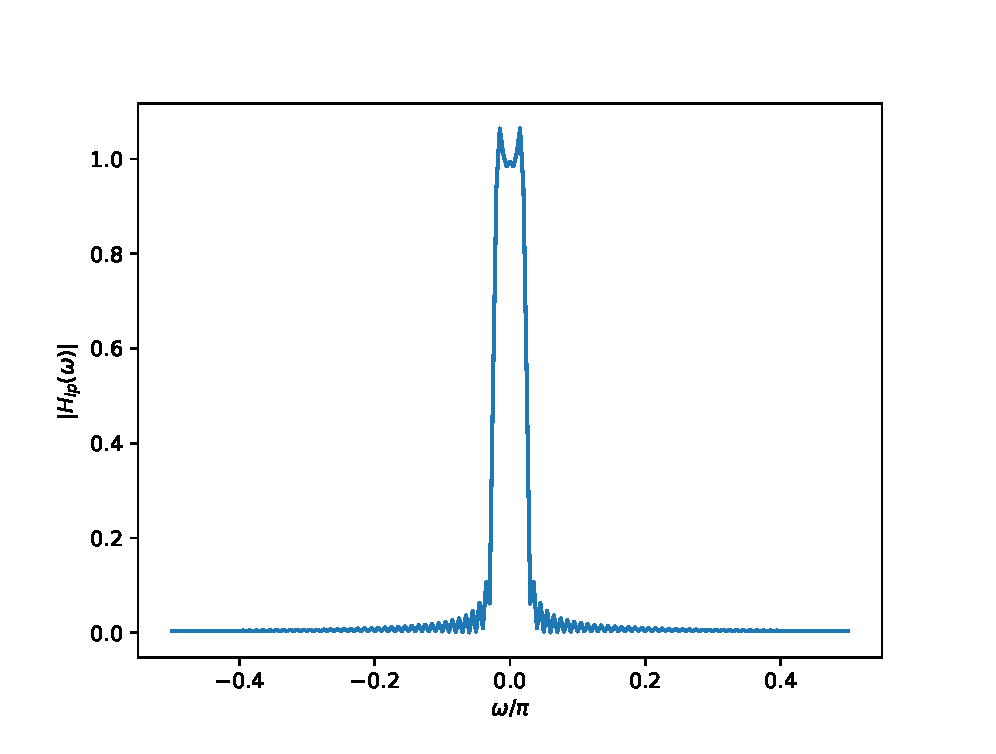
\includegraphics[width = 15cm]{figs/fir/lowpass.eps}
\caption{The magnitude response of the FIR lowpass digital filter designed to meet the given specifications} 
\end{figure}

\subsection{The FIR Bandpass Filter}
The centre of the passband of the desired bandpass filter was found to be $\omega_c = 0.275\pi$ in Section
2.1.  The impulse response of the desired bandpass filter is obtained from the impulse response of the
corresponding lowpass filter as
\begin{eqnarray}
h_{bp}(n) = 2h_{lp}(n)cos(n\omega_c)
\end{eqnarray}
Thus, from (\ref{firlpfinal}), we obtain
\begin{eqnarray}
\label{firbpfinal}
h_{bp}(n) &=& \frac{2\sin(\frac{n\pi}{40}) \cos(\frac{11n\pi}{40})}{n\pi} \indent -100 \leq n \leq 100 \nonumber \\
&=& 0, \hspace{4cm} \mbox{otherwise}
\end{eqnarray}
%
The magnitude response of the FIR bandpass filter designed to meet the given specifications is plotted in Figure 6.
\begin{figure}
\label{fig6}
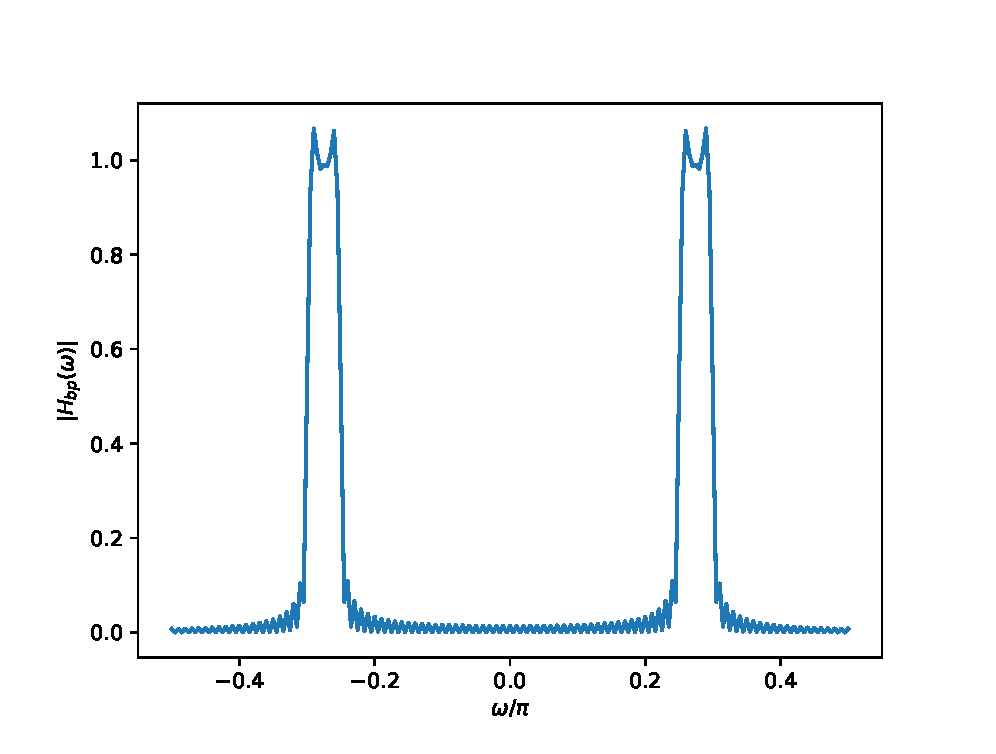
\includegraphics[width = 15cm]{figs/fir/bandpass.eps}
\caption{The magnitude response of the FIR bandpass digital filter designed to meet the given specifications} 
\end{figure}

\end{document}
